\documentclass[border=20pt]{standalone}
\usepackage{amsmath}
\usepackage{graphicx}
\usepackage{helvet}
\renewcommand{\familydefault}{\sfdefault}

\usetikzlibrary{
    positioning,
    arrows.meta,
    shapes,
    shapes.multipart,
    fit,
    backgrounds
}

\begin{document}

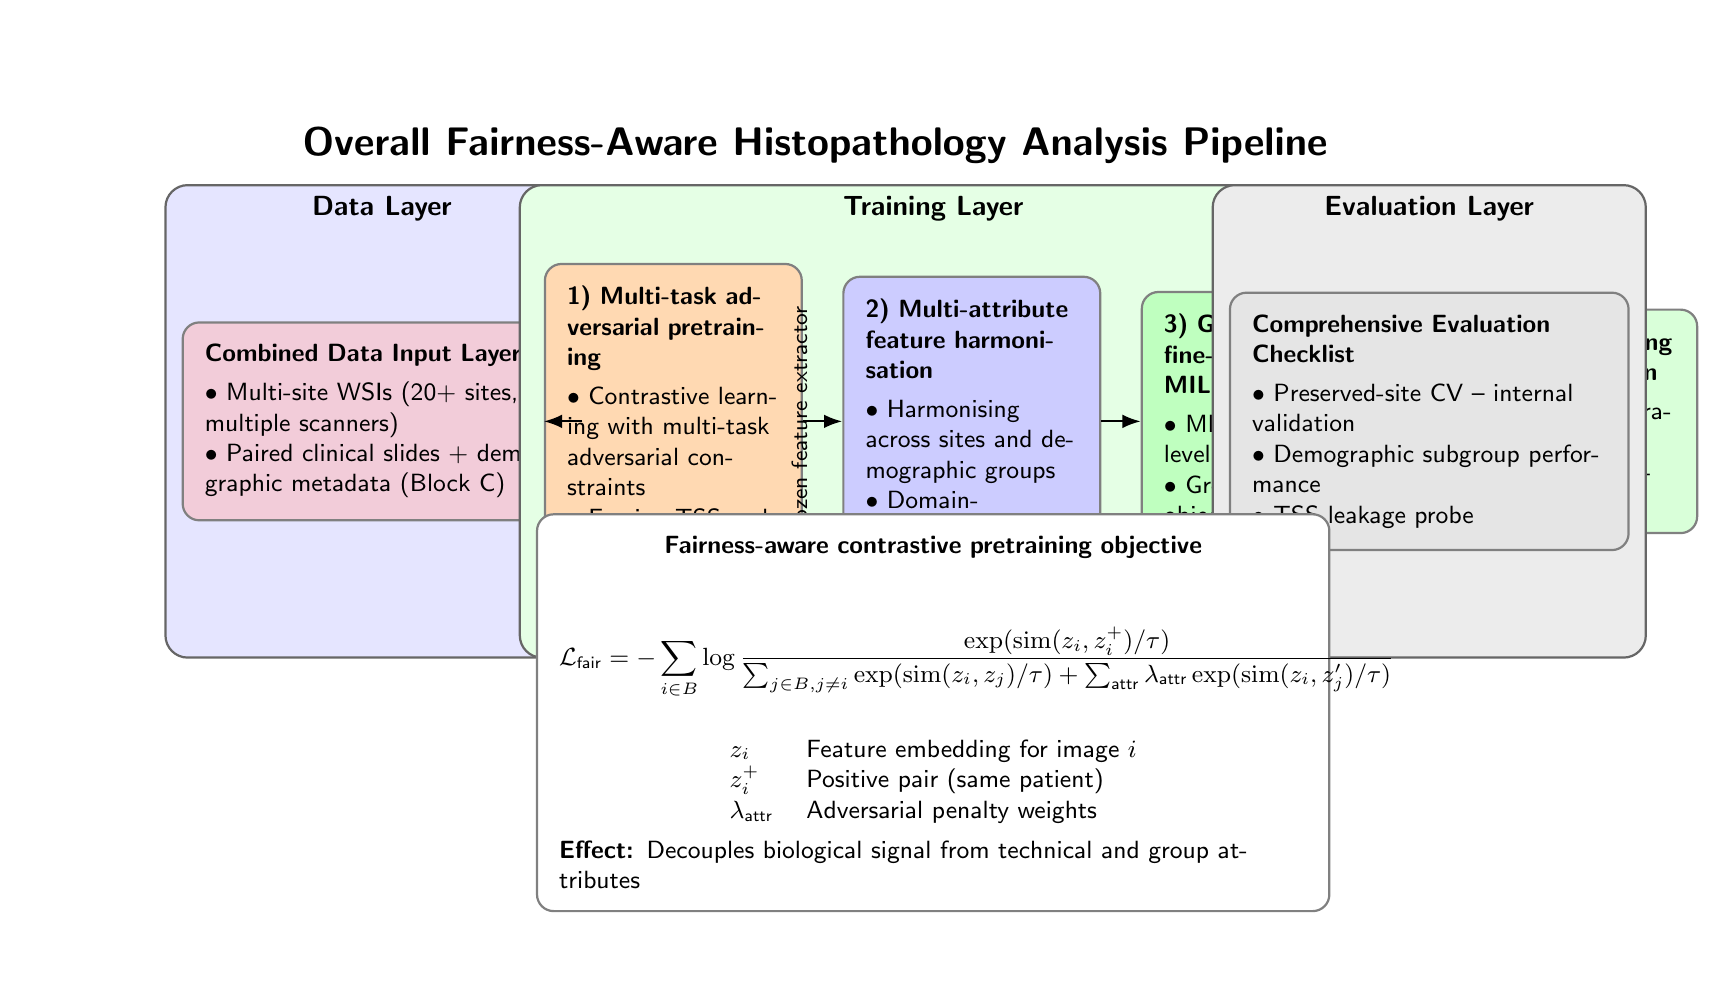
\begin{tikzpicture}[
    font=\small,
    box/.style={
        rounded corners=6pt,
        draw=black!50,
        thick,
        align=left,
        inner sep=8pt
    },
    layer/.style={
        rounded corners=8pt,
        draw=black!60,
        thick,
        inner sep=10pt
    },
    arrow/.style={-Latex, thick}
]

% Set bounding box to ensure all content is visible
\useasboundingbox (-2,-1) rectangle (19,11);

% ================= TITLE =================
\node[font=\Large\bfseries] at (8,9.5)
{Overall Fairness-Aware Histopathology Analysis Pipeline};

% ================= DATA LAYER =================
\node[layer, fill=blue!10, minimum width=5.5cm, minimum height=6cm] (data) at (2.5,6)
{};

\node[font=\bfseries] at (2.5,8.7) {Data Layer};

\node[box, fill=purple!20, text width=4.5cm] (input) at (2.5,6) {
\textbf{Combined Data Input Layer}

\vspace{3pt}
$\bullet$ Multi-site WSIs (20+ sites, multiple scanners)

$\bullet$ Paired clinical slides + demographic metadata (Block C)
};

% ================= TRAINING LAYER =================
\node[layer, fill=green!10, minimum width=10.5cm, minimum height=6cm] (train) at (9.5,6)
{};
\node[font=\bfseries] at (9.5,8.7) {Training Layer};

% ---- Box 1
\node[box, fill=orange!30, text width=2.7cm] (b1) at (6.2,6) {
\textbf{1) Multi-task adversarial pretraining}

\vspace{3pt}
$\bullet$ Contrastive learning with multi-task adversarial constraints

$\bullet$ Forcing TSS and attribute invariance
};

% ---- Box 2
\node[box, fill=blue!20, text width=2.7cm, right=0.5cm of b1] (b2) {
\textbf{2) Multi-attribute feature harmonisation}

\vspace{3pt}
$\bullet$ Harmonising across sites and demographic groups

$\bullet$ Domain-adversarial learning
};

% ---- Box 3
\node[box, fill=green!25, text width=2.7cm, right=0.5cm of b2] (b3) {
\textbf{3) Group-specific fine-tuning (FairMIL)}

\vspace{3pt}
$\bullet$ MIL for patient-level prediction

$\bullet$ Group-sensitive objective
};

% ---- Box 4
\node[box, fill=green!15, text width=2.7cm, right=0.5cm of b3] (b4) {
\textbf{4) Post-processing model calibration}

\vspace{3pt}
$\bullet$ Subgroup calibration

$\bullet$ Equalizing metrics
};

% ================= ARROWS =================
\draw[arrow] (input.east) -- (b1.west);
\draw[arrow] (b1.east) -- (b2.west);
\draw[arrow] (b2.east) -- (b3.west);
\draw[arrow] (b3.east) -- (b4.west);

\node[rotate=90] at (7.8,6) {\footnotesize frozen feature extractor};

% ================= EVALUATION =================
\node[layer, fill=gray!15, minimum width=5.5cm, minimum height=6cm] (eval) at (15.8,6)
{};
\node[font=\bfseries] at (15.8,8.7) {Evaluation Layer};

\node[box, fill=gray!20, text width=4.5cm] (evalbox) at (15.8,6) {
\textbf{Comprehensive Evaluation Checklist}

\vspace{3pt}
$\bullet$ Preserved-site CV – internal validation

$\bullet$ Demographic subgroup performance

$\bullet$ TSS leakage probe
};

% ================= EQUATION PANEL =================
\node[box, fill=white, minimum width=10cm, text width=9.5cm] (eq) at (9.5,2.3)
{
\centering
\textbf{Fairness-aware contrastive pretraining objective}

\vspace{6pt}

\[
\mathcal{L}_{\text{fair}} =
- \sum_{i \in B}
\log
\frac{
\exp(\mathrm{sim}(z_i, z_i^+)/\tau)
}{
\sum_{j \in B, j \neq i}
\exp(\mathrm{sim}(z_i, z_j)/\tau)
+
\sum_{\text{attr}} \lambda_{\text{attr}}
\exp(\mathrm{sim}(z_i, z_j')/\tau)
}
\]

\vspace{4pt}

\begin{tabular}{ll}
$z_i$ & Feature embedding for image $i$ \\
$z_i^+$ & Positive pair (same patient) \\
$\lambda_{\text{attr}}$ & Adversarial penalty weights \\
\end{tabular}

\vspace{4pt}

\textbf{Effect:} Decouples biological signal from technical and group attributes
};

\end{tikzpicture}

\end{document}
